\documentclass[12pt, letterpaper]{article}

% --- Paquetes Necesarios ---
\usepackage[utf8]{inputenc}
\usepackage[spanish, es-tabla]{babel}
\usepackage[margin=2.5cm]{geometry}
\usepackage{graphicx}
\usepackage{tabularx}
\usepackage{titlesec}
\usepackage{hyperref}
\usepackage{tocloft} % Para personalizar el índice
\usepackage{tabularx}
\usepackage{colortbl}
\usepackage[table]{xcolor}
\usepackage[utf8]{inputenc}
\usepackage[T1]{fontenc}
\usepackage[spanish]{babel}
\usepackage{tabularx}
\usepackage{multirow}
\usepackage{array}

\usepackage[a4paper,margin=2.5cm]{geometry}
\definecolor{javBlue}{RGB}{0,57,107}
\definecolor{lightgray2}{RGB}{245,245,245}
\definecolor{headergray}{RGB}{230,230,230}


\usepackage{graphicx}
\usepackage{float}
\usepackage{array}
\usepackage{longtable}
\usepackage{tabularx}
\usepackage{booktabs}
\usepackage{multirow}
\usepackage{xcolor}
\usepackage{colortbl}
\usepackage{caption}
\usepackage{parskip}
\usepackage{enumitem}
\usepackage{amsmath}
\usepackage{hyperref}
\usepackage{tikz}
\usetikzlibrary{
    positioning,
    arrows.meta,
    shapes.geometric,
    calc
}
\setlength{\tabcolsep}{6pt}
\renewcommand{\arraystretch}{1.35}

\newcolumntype{Y}{>{\raggedright\arraybackslash}X}
% --- Configuración del Índice (TOC) ---
% Asegura que las sub-subsecciones aparezcan en el índice
\setcounter{tocdepth}{3}
\setcounter{secnumdepth}{3}

% --- Configuración de Formato ---
\hypersetup{
    colorlinks=true,
    linkcolor=black,
    urlcolor=blue,
}

% ============================================================
% TABLA DE REQUERIMIENTOS NO FUNCIONALES
% ============================================================

\newenvironment{reqtable}
{
\renewcommand{\arraystretch}{1.4}
\begin{longtable}{|
>{\raggedright\arraybackslash\bfseries}p{3cm}|
>{\raggedright\arraybackslash}p{11cm}|
}
\hline
\rowcolor{headergray}
\textbf{Código} & \textbf{Descripción} \\ \hline
\endhead
}
{
\end{longtable}
}

\newcommand{\reqrow}[2]
{
#1 & #2 \\ \hline
}

\newcommand{\reqrowgray}[2]
{
\rowcolor{lightgray2}
#1 & #2 \\ \hline
}

% --- Inicio del Documento ---
\begin{document}

% --- Portada ---
\begin{titlepage}
    \centering
    \vspace*{1cm}
    {\Huge \textbf{GammaLab V2.0}} \\[0.5cm]
    {\Large Pontificia Universidad Javeriana} \\[2cm]
    \textbf{ESPECIFICACIÓN DE REQUERIMIENTOS DE SOFTWARE} \\[3cm]
    
\includegraphics[width=4cm]{logo.png} \\[2cm]
    \textbf{Autores:} \\ Juan Felipe Romero Ortiz \\ Laura Juliana Garzón Arias \\  Xiomara Herrera Suárez \\ Sebastián Almanza Galvis \\[2cm]
    \textbf{Fecha:} 23/05/2026 \\
    \textbf{Versión:} v1.0
    \vfill
\end{titlepage}

% --- 1. Historial de Cambios (Página 1) ---
\newpage
\pagenumbering{arabic}
\section*{HISTORIAL DE CAMBIOS}
\addcontentsline{toc}{section}{HISTORIAL DE CAMBIOS}
\begin{table}[h!]
\centering
\small
\begin{tabularx}{\textwidth}{|l|l|X|X|X|}
\hline
\textbf{Versión} & \textbf{Fecha} & \textbf{Sección} & \textbf{Descripción} & \textbf{Responsable} \\ \hline
v1.0 & 17/05/26 inicio del documento & Se inició la creación del SRS y se dividió el trabajo para cada persona & Juan Felipe Romero Ortiz, Laura Juliana Garzón Arias,  Xiomara Herrera Suárez, Sebastián Almanza Galvis \\ \hline
\end{tabularx}
\caption{Historial de cambios}
\end{table}

% --- 2. Contenido / Índice (Página 2) ---
\newpage
\renewcommand{\contentsname}{CONTENIDO}
\addcontentsline{toc}{section}{CONTENIDO}
\tableofcontents

% --- 3. Listas (Página 4 y 5) ---
\newpage
\addcontentsline{toc}{section}{LISTA DE TABLAS}
\listoftables

\newpage
\addcontentsline{toc}{section}{LISTA DE ILUSTRACIONES}
\listoffigures

% --- 4. Cuerpo del Documento (Página 6 en adelante) ---
\newpage
\section{INTRODUCCIÓN}
\subsection{Propósito}

El presente documento constituye la Especificación de Requisitos de Software (SRS) de GammaLab 2.0. Con el proposito de brindar una orientación metodológica clara del inicio del ciclo de desarrollo.
% Producto -----------------------------------------------------------------------
GammaLab v2.0 es una interfaz gráfica de escritorio de tipo standalone orientada al análisis, procesamiento y visualización de señales electroencefalográficas o EEG. Concebido como una alternativa de código abierto y enfocado en el uso local para el Laboratorio de Electrofisiología de la Universidad de Colombia, el sistema está desarrollado con el lenguaje Python, utilizando el framework PySide6 y librerías científicas como VTK. Siguiendo con la visión de GammaLab v1.0, su diseño arquitectónico evoluciona con el fin de resolver brechas en el paralelismo de cómputo y añadir nuevos métodos de acoplamiento cruzado de frecuencias (Phase-Amplitude-Coupling o PAC).

% Alcanse del SRS -----------------------------------------------------------------
Este documento especifica de manera formal, atómica y verificable la totalidad de los requerimientos funcionales y no funcionales que rigen el desarrollo de GammaLab v2.0. El alcance de este abarca detalladamente los requerimientos de interfaz de usuario, gestión de memoria DataStore, el procesamiento asíncrono en segundo plano del Kernel y las especificaciones técnicas del nuevo módulo de análisis (PAC). Se excluye del alcance del SRS las rutas de mantenimiento técnico a largo plazo del software, así mismo el código heredado de GammaLab v1.0 que se conservará sin modificaciones funcionales.

% Audiencia -----------------------------------------------------------------------
La audiencia de este documento comprende cuatro grupos: el equipo de desarrollo, que lo utilizará como referencia técnica durante el diseño y la implementación; la directora del proyecto, en su rol de Product Owner, quien lo empleará para validar que el alcance acordado se mantenga a lo largo del desarrollo; el Laboratorio de Señales de la Universidad Nacional de Colombia, como cliente y usuario final del sistema; y los evaluadores académicos del proyecto de grado, ante quienes el documento evidencia el rigor metodológico del proceso de ingeniería seguido.

% "Importancia" le falta -----------------------------------------------------------
La importancia de este SRS radica en que este actúa como puente de información oficial entre las necesidades del laboratorio y la implementación técnica del software. Al definir los criterios de medición para cada funcionalidad y asociarlos a los requerimientos, el documento mitiga el riesgo de ambigüedad técnica. Por último, este texto sirve como un instrumento principal de trazabilidad y verificación que, a lo largo del ciclo de vida del proyecto, garantice que cada incremento dentro del software responda de forma adecuada a las necesidades previamente acordadas.

\subsubsection{Contexto - GammaLab v1.0}

% Origen de GammaLab 1 -------------------------------------------------------------
GammaLab nació en 2025 como una alternativa de código abierto a las herramientas con licencia comercial y fragmentada en el mercado, enfocada específicamente en las necesidades del Laboratorio de Electrofisiología de la Universidad Nacional de Colombia. El sistema se estructuró bajo una arquitectura microkernel con un ecosistema de plugins usando Python, permitiendo el análisis de señales EEG en los dominios de tiempo, frecuencia y tiempo-frecuencia mediante una interfaz gráfica unificada.

Aunque la primera iteración fue validada exitosamente con un 87.5\% de coincidencia frente al sistema de referencia BOARD-FTD-PACC, las pruebas de aceptación con el usuario final  identificaron brechas críticas para su correcta adopción. Entre estas limitaciones se destacan la ausencia de persistencia de sesiones y gestión de proyectos, la falta de rendimiento al no contar con mecanismos de concurrencia o paralelismo para la distribución de tareas pesadas.

% Necesidad de GammaLab2 -----------------------------------------------------------
Además, el equipo de investigación reportó la necesidad de contar con un control más preciso sobre la densidad de muestreo y la incorporación de métodos analíticos avanzados. Por otro lado, GammaLab v2.0 se concibe más allá de solo extender estas capacidades, sino para estabilizar la arquitectura meidnate el procesamiento asíncrono en segundo plano, así garantizando la robustez técnica necesaria para los investigadores.

\subsection{Alcance}
El alcance de GammaLab v2.0 lo definen los límites funcionales, técnicos y operativos del sistema, asegurando la entrega de un software robusto y enfocado en el entorno de investigación. 

% Descripción del producto ------------------
GammaLab v2.0 se define como una aplicación de escritorio standalone, lo que significa que es local y funcional sin acceso a internet. Desarrollada en el lenguaje Python bajo el framework PySide6 y librerías de visualización científicas VTK. El sistema está diseñado específicamente para interactuar con archivos de señales electroencefalográficas (EEG) en formatos estándar como ABF, EDF, BDF y MAT. Su arquitectura está diseñada para investigadores y estudiantes del Laboratorio de Electrofisiología de la Universidad Nacional de Colombia, permitiéndoles ejecutar análisis avanzados sin requerir conocimientos en programación, ni fragmentando su flujo de trabajo en diferentes herramientas durante sus análisis.
% Funcionalideades ------------------
Con el fin de cerrar las brechas observadas de la primera iteración del software, la visión de esta segunda iteración se definirá por medio de las siguientes funciones:

\textbf{Funcionalidades adicionales}
\begin{itemize}

\item \textbf{Persistencia de sesión y gestión de proyectos:} Implementación del componente ProjectSession para permitir el guardado local, creando una extensión propia para GammaLab (.glab) y la restauración automática del entorno de trabajo.

\item \textbf{Kernel de procesamiento asíncrono y paralelo:} Desacoplamiento de la interfaz de usuario mediante una arquitectura de multiprocesamiento para la ejecución paralela del análisis matemático pesado en segundo plano sin congelar la GUI.

\item \textbf{Módulo de análisis PAC:} Incorporación del un plugin especializado para cuantificar el acoplamiento phase-amplitude coupling, permitiendo la selección cruzada de canales fuentes.

\item \textbf{Optimización visual y gráfica vectorial:} Inclusión de técnicas de submuestreo de señal dinámica para navegación fluida (>= 24 FPS) y soporte de exportación gráfica en alta calidad mediante el formato EMF.

\end{itemize}

% fuer ad ealcance -------------------
\textbf{Funcionalidades excluidas (fuera de alcance)}
\begin{itemize}

\item El sistema no implementará almacenamiento de datos en la nube, sincronización web o bases de datos compartidas. Todo análisis ejecutado en la aplicación se realizará de forma local en el disco duro del usuario.

\item El sistema no incluye módulos para la adquisición de señales EEG en tiempo real mediante conexiones físicas a amplificadores o diademas de electrodos.

\item Se excluye el soporte para el procesamiento de otro tipo de bioseñales; el soporte es exclusivo de señales electroencefalográficas.

\end{itemize}

% Utilidades ------------------
El desarrollo de esta evolución funcional y arquitectónica aporta tres aspectos claves para el ecosistema del laboratorio:

\begin{itemize}
    \item \textbf{Análisis avanzado:} Al generar un entorno puramente visual para métricas complejas de acoplamiento cruzado de secuencias, se elimina la fricción técnica de programar algoritmos desde cero.
    \item \textbf{Soberanía tecnológica y sostenibilidad financiera:} Al ser una alternativa sólida de código abierto bajo la licencia MIT, el laboratorio elimina dependencias de licencias costosas o plataformas comerciales cerradas.

    \item \textbf{Eficiencia computacional:} La paralelización del kernel reduce drásticamente los tiempos de procesamiento de grandes volúmenes de datos, optimizando los tiempos de respuesta del programa.
\end{itemize}

% Relación con el contexto organizacional ------------------
El laboratorio suele tener nulo mantenimiento técnico especializado para software. Por lo tanto, el diseño de GammaLab v2.0 se alinea con la meta de entregar una herramienta autónoma, autogestionable y autoexplicativa. EL despliegue mediante un instalador ejecutable de un solo clic y la incorporación de ayudas contextuales (tooltips) robustas garantizan que el laboratorio pueda usar la herramienta de manera independiente, apoyando en sus proyectos de investigación.

\subsection{Definiciones, Acrónimos y Abreviaciones}
\begin{table}[ht]
\centering
\renewcommand{\arraystretch}{1.1}
\small

\begin{tabular}{|p{4cm}|p{10cm}|}
\hline
\textbf{Acrónimo / Abreviación} & \textbf{Definición} \\ \hline

\textbf{EEG} & Electroencefalografía (\textit{Electroencephalography}). \\ \hline

\textbf{GUI} & Interfaz gráfica de usuario (\textit{Graphical User Interface}). \\ \hline

\textbf{ERP} & Potencial relacionado a eventos (\textit{Event Related Potential}). \\ \hline

\textbf{FFT} & Transformada Rápida de Fourier (\textit{Fast Fourier Transform}). \\ \hline

\textbf{PSD} & Densidad Espectral de Potencia (\textit{Power Spectral Density}). \\ \hline

\textbf{PAC} & Acoplamiento fase-amplitud (\textit{Phase-Amplitude Coupling}). \\ \hline

\textbf{VTK} & Visualization Toolkit. Librería de visualización científica 2D y 3D. \\ \hline

\textbf{CSV} & Valores separados por comas (\textit{Comma-Separated Values}). \\ \hline

\textbf{XLSX} & Formato de hoja de cálculo basado en Office Open XML utilizado por Microsoft Excel. \\ \hline

\textbf{PNG} & Portable Network Graphics. \\ \hline

\textbf{JPG} & Joint Photographic Experts Group. \\ \hline

\textbf{EMF} & Enhanced Metafile Format. \\ \hline

\textbf{ABF} & Axon Binary File. \\ \hline

\textbf{EDF} & European Data Format. \\ \hline

\textbf{BDF} & BioSemi Data Format. \\ \hline

\textbf{MAT} & Formato de archivo de MATLAB. \\ \hline

\textbf{RAM} & Random Access Memory. \\ \hline

\textbf{VRAM} & Video Random Access Memory. \\ \hline

\textbf{CPU} & Central Processing Unit. \\ \hline

\textbf{I/O} & Input/Output. \\ \hline

\textbf{UX} & User Experience. \\ \hline

\textbf{SRS} & Software Requirements Specification. \\ \hline

\textbf{PMP} & Project Management Plan. \\ \hline

\end{tabular}

\caption{Acrónimos y abreviaciones en el SRS}

\end{table}

\newpage

\subsection{Referencias}

\renewcommand{\refname}{}

\renewcommand{\refname}{\vspace{-2 em}} 

\begin{thebibliography}{12}

\bibitem{ref1}
Microsoft Corporation, ``Windows -- product family overview,'' Available: \url{https://www.microsoft.com/windows}. Accessed: 2025.

\bibitem{ref2}
Python Software Foundation, ``The Python tutorial --- Python 3.11 documentation,'' 2023. Available: \url{https://docs.python.org/3/tutorial/index.html}. Accessed: 2025.

\bibitem{ref3}
Riverbank Computing, ``PyQt --- Python bindings for Qt,'' 2025. Available: \url{https://www.riverbankcomputing.com/software/pyqt/}. Accessed: 2025.

\bibitem{ref4}
Kitware, ``The Visualization Toolkit (VTK),'' 2025. Available: \url{https://vtk.org/}. Accessed: 2025.

\bibitem{ref5}
NumPy Developers, ``NumPy documentation,'' 2025. Available: \url{https://numpy.org/doc/stable/}. Accessed: 2025.

\bibitem{ref6}
SciPy Community, ``SciPy --- fundamental algorithms for scientific computing in Python,'' 2025. Available: \url{https://scipy.org/}. Accessed: 2025.

\bibitem{ref7}
The pandas Development Team, ``pandas --- Python data analysis library,'' 2025. Available: \url{https://pandas.pydata.org/}. Accessed: 2025.

\bibitem{ref8}
G. R. Lee, R. Gommers, F. Wasilewski, K. Wohlfahrt, and A. O'Leary, ``PyWavelets: A Python package for wavelet analysis,'' \textit{Journal of Open Source Software}, vol. 4, no. 36, p. 1237, 2019. Available: \url{https://doi.org/10.21105/joss.01237}.

\bibitem{ref9}
S. W. Harden, ``pyabf 2.3.5,'' 2022. Available: \url{https://pypi.org/project/pyabf/}.

\bibitem{ref10}
Teunis van Beelen, ``pyEDFlib,'' 2025. Available: \url{https://pypi.org/project/pyEDFlib/}. Accessed: 2025.

\bibitem{ref11}
Python Software Foundation, ``concurrent.futures --- launching parallel tasks,'' 2025. Available: \url{https://docs.python.org/3/library/concurrent.futures.html}. Accessed: 2025.

\bibitem{ref12}
pytest Development Team, ``pytest documentation,'' 2025. Available: \url{https://docs.pytest.org/en/stable/}. Accessed: 2025.

\end{thebibliography}
\subsection{Apreciación Global}

Este documento especifica los requerimientos de software de GammaLab 2.0, abarcando desde la descripción general del sistema hasta la definición detallada de sus requerimientos funcionales y no funcionales. Se organiza en tres bloques principales: una descripción general que contextualiza el producto, sus usuarios y las condiciones bajo las cuales opera; la especificación de requerimientos funcionales, organizada por módulo; y los requerimientos no funcionales junto con los procesos de ingeniería y verificación aplicados. Cada sección cumple un rol específico: los requerimientos funcionales y no funcionales orientan las decisiones de diseño e implementación, mientras que el modelo del dominio y la distribución de requerimientos permiten mantener una comprensión uniforme del sistema entre todos los involucrados.

\newpage



\newpage

\section{DESCRIPCIÓN GLOBAL}

\subsection{Perspectiva del Producto}

GammaLab 2.0 es una aplicación de escritorio standalone para análisis y
visualización de señales neurofisiológicas (EEG), ejecutada localmente en
estaciones de trabajo con Windows 10 o superior. El sistema mantiene una
arquitectura modular orientada a plugins, donde un Kernel interno (IoC)
orquesta servicios comunes como el almacenamiento de procesamientos, la
gestión de eventos y la ejecución de tareas.

La aplicación no introduce dependencias de red ni bases de datos externas.
GammaLab 2.0 pertenece a una familia de productos: es la segunda versión de
GammaLab 1.0, desarrollada en la Pontificia Universidad Javeriana bajo la
dirección de la misma directora y orientada al mismo cliente, el Laboratorio
de Señales de la Universidad Nacional de Colombia.

Sobre la versión anterior, esta versión incorpora mejoras en la experiencia
de usuario, persistencia y restauración de proyectos, una estrategia de
paralelización del procesamiento implementada en el Kernel y un nuevo módulo
de análisis basado en acoplamiento cruzado de frecuencias
(\textit{Cross-Frequency Coupling}).

El nuevo módulo incluye el análisis de acoplamiento fase-amplitud
(\textit{Phase-Amplitude Coupling}, PAC) sobre un canal, PAC entre dos
canales y coherencia de fase (PPC). GammaLab 2.0 es compatible con los
archivos y flujos de trabajo de su versión original.

\subsubsection{Interfaces con el Sistema}

GammaLab 2.0 no se integra con sistemas externos ni servicios en la nube.
Su operación es completamente local y su contexto es el procesamiento de
archivos de señales EEG adquiridos previamente con herramientas externas.

Las interfaces con el entorno son de dos tipos: interfaces de archivo para la
entrada y salida de señales, e interfaces de usuario a través de la GUI, sin
intercambio de mensajes con servicios remotos.

La comunicación entre los plugins y el Kernel del sistema se realiza a través
del contrato de integración definido en la arquitectura interna. La
paralelización opera dentro del Kernel, que puede ejecutar tareas mediante
hilos para operaciones de entrada y salida o mediante procesos independientes
para cálculos intensivos.

\subsubsection{Interfaces con el Usuario}

Se describen los medios de interacción previstos y sus características
técnicas:

\begin{itemize}

    \item \textbf{Teclado.} Entrada de datos en formularios para la
    definición de parámetros como frecuencia de muestreo, rangos de
    frecuencias, selección de canales, selección de trials y demás
    parámetros requeridos por los módulos de análisis.

    \item \textbf{Ratón/Trackpad.} Navegación y control de la GUI: selección
    de botones, menús, pestañas, canales, trials e interacción con gráficas.

    \item \textbf{Pantalla.} Visualización de la interfaz, pestañas y
    gráficos generados por cada módulo. Especificaciones: resolución mínima
    1920 x 1080 px; tamaño recomendado mayor o igual a 14 pulgadas.

    \item \textbf{Interfaz gráfica (GUI).} Desarrollada en Python con
    PySide6 y los componentes Qt. Está organizada en módulos navegables con
    barras laterales para la selección de la señal activa, la configuración
    de parámetros por plugin, la ejecución de análisis y la visualización
    de resultados. GammaLab 2.0 incorpora las vistas de PAC de un canal, PAC
    inter-canal y coherencia de fase.

    \item \textbf{Interfaz de entrada de archivos EEG.} Permite al usuario
    seleccionar y cargar archivos de señales adquiridos externamente en los
    formatos \texttt{.abf}, \texttt{.edf}, \texttt{.bdf} y \texttt{.mat},
    mediante el selector de archivos nativo de Windows.

\end{itemize}

\subsubsection{Interfaces con el Hardware}

GammaLab 2.0 no establece comunicación directa con equipos de adquisición de
señales ni utiliza protocolos de red o puertos de comunicación, dado que
opera exclusivamente de manera local sobre archivos previamente adquiridos.

La interacción con hardware se limita a dispositivos estándar de entrada,
como teclado, ratón y trackpad, y de salida, como la pantalla. Durante la
ejecución, los datos del sistema se almacenan temporalmente en memoria RAM y
las tareas de procesamiento pueden distribuirse entre varios núcleos.

\subsubsection{Interfaces con el Software}

\begin{itemize}

    \item \textbf{Windows.} Es el sistema operativo base sobre el que se
    ejecuta GammaLab 2.0. Se requiere Windows 10 de 64 bits o superior
    \cite{ref1}.

    \item \textbf{Python.} Es el lenguaje de programación base del sistema.
    Se utiliza la versión 3.11--3.12 \cite{ref2}.

    \item \textbf{PySide6.} Es el framework sobre el que se construye la
    interfaz gráfica del sistema, manejando widgets, layouts, navegación y
    eventos mediante los componentes Qt \cite{ref3}.

    \item \textbf{VTK.} Es la librería utilizada para el renderizado
    embebido de señales EEG y la visualización científica 2D y 3D dentro de
    la aplicación\cite{ref4}.

    \item \textbf{NumPy.} Provee las estructuras de arreglos
    multidimensionales y las operaciones matemáticas base del sistema,
    incluyendo las operaciones requeridas por los análisis espectrales y el
    análisis de acoplamiento cruzado de frecuencias.

    \item \textbf{SciPy.} Complementa a NumPy con módulos especializados para
    procesamiento de señales, incluyendo el cálculo de densidad espectral de
    potencia, interpolaciones y filtros como Butterworth \cite{ref6}.

    \item \textbf{MNE.} Proporciona herramientas especializadas para el
    procesamiento y análisis de señales neurofisiológicas.

    \item \textbf{TensorPAC.} Proporciona algoritmos para el cálculo del
    acoplamiento fase-amplitud, la generación de comodulogramas, histogramas
    de fase y vectores de acoplamiento medio.

    \item \textbf{Pandas.} Gestiona la organización y exportación de
    resultados en formatos tabulares como \texttt{.csv}, \texttt{.xlsx} y
    \texttt{.json} \cite{ref7}.

    \item \textbf{PyWavelets.} Provee los algoritmos para el cálculo de la
    transformada wavelet y su promedio en el dominio tiempo-frecuencia.

    \item \textbf{pyABF.} Permite la lectura de archivos de
    electrofisiología en formato \texttt{.abf} \cite{ref9}.

    \item \textbf{pyEDFlib.} Permite la lectura de archivos de
    electrofisiología en formato \texttt{.edf} \cite{ref10}.

    \item \textbf{concurrent.futures y multiprocessing.} Son módulos de la
    biblioteca estándar de Python utilizados para implementar la
    paralelización en el Kernel. Permiten distribuir las tareas entre hilos
    para operaciones de entrada y salida y entre procesos independientes para
    cálculos intensivos \cite{ref11}.

    \item \textbf{pytest.} Es el framework utilizado para la validación
    interna del sistema mediante pruebas unitarias, cubriendo módulos de
    carga de señales, filtrado, generación de trials, análisis PAC,
    análisis inter-canal, exportación y ejecución paralela de tareas \cite{ref11}.

\end{itemize}

\subsubsection{Interfaces de Comunicación}

GammaLab 2.0 no utiliza interfaces de comunicación de red. El sistema no
implementa protocolos como TCP/IP, HTTP, sockets ni buses de mensajería, y no
requiere conexión a redes locales o remotas para su operación.

Todo el procesamiento ocurre localmente en el equipo del usuario, sin
intercambio de datos con sistemas externos.

\subsubsection{Restricciones de Memoria}

\begin{itemize}

    \item \textbf{Entorno Python.} GammaLab 2.0 se desarrolla en Python
    3.11+, requiriendo espacio en disco para el entorno base y sus
    dependencias.

    \item \textbf{Librerías Científicas.} El uso de NumPy, SciPy, MNE,
    Pandas, TensorPAC y PyWavelets genera un consumo adicional de memoria
    durante el procesamiento de señales EEG, dependiendo del tamaño de los
    arreglos manipulados y del número de trials seleccionados.

    \item \textbf{Interfaz Gráfica.} La GUI construida con PySide6 demanda
    memoria adicional durante la ejecución, especialmente cuando se
    visualizan simultáneamente varias gráficas y resultados.

    \item \textbf{Visualización Científica.} Las operaciones de renderizado
    mediante VTK pueden incrementar el consumo de RAM y VRAM dependiendo de
    la cantidad de señales y resultados visualizados.

    \item \textbf{Lectura de Archivos EEG.} Las librerías pyEDFlib y pyABF
    presentan un consumo variable según la cantidad de canales y puntos de
    cada señal.

    \item \textbf{Paralelización del Kernel.} La ejecución simultánea de
    tareas mediante \textit{multiprocessing} implica la creación de procesos
    independientes, cada uno con su propio espacio de memoria. En escenarios
    de carga alta, esto puede incrementar el consumo total de RAM de acuerdo
    con el número de procesos activos.

\end{itemize}

Con base en lo anterior, se definen los siguientes requerimientos de
hardware:

\subsubsection*{Requerimientos mínimos}

\begin{itemize}
    \item \textbf{Procesador:} CPU de 4 núcleos a 2.0 GHz o superior
    (AMD Ryzen 3 / Intel i3).
    \item \textbf{RAM:} 8 GB.
    \item \textbf{VRAM:} 1 GB (GPU integrada).
    \item \textbf{Almacenamiento:} 3 GB libres.
\end{itemize}

\subsubsection*{Requerimientos recomendados}

\begin{itemize}
    \item \textbf{Procesador:} CPU de 4--8 núcleos a 3.0 GHz o superior
    (AMD Ryzen 5 / Intel i5 o superior).
    \item \textbf{RAM:} 16 GB.
    \item \textbf{VRAM:} 2 GB.
    \item \textbf{Almacenamiento:} 20 GB libres en SSD.
\end{itemize}

\subsubsection{Operaciones}

Durante su uso, GammaLab 2.0 permite al usuario realizar las siguientes
operaciones principales:

\begin{itemize}

    \item \textbf{Cargar señal.} Seleccionar y cargar archivos de señal en
    formatos \texttt{.abf}, \texttt{.edf}, \texttt{.bdf} y \texttt{.mat}.

    \item \textbf{Preprocesamiento.} Dividir la señal en trials, eliminar
    artefactos de estimulación y aplicar filtros como Butterworth.

    \item \textbf{Análisis.} Procesar la señal en los dominios de tiempo,
    frecuencia y tiempo-frecuencia, incluyendo FFT, PSD, Wavelet, ERP,
    análisis PAC de un canal, PAC inter-canal y coherencia de fase PPC.

    \item \textbf{Análisis PAC.} Seleccionar bandas de fase y amplitud,
    seleccionar un trial o un promedio de trials, calcular el
    acoplamiento fase-amplitud y visualizar sus resultados.

    \item \textbf{Análisis inter-canal.} Seleccionar un canal como fuente de
    fase y otro como fuente de amplitud para calcular PAC inter-canal o
    coherencia de fase PPC.

    \item \textbf{Visualización y exportación.} Visualizar los resultados del
    procesamiento y exportarlos en formatos numéricos y gráficos como
    \texttt{.csv}, \texttt{.xlsx}, \texttt{.json}, \texttt{.jpeg},
    \texttt{.jpg}, \texttt{.png} y \texttt{.tiff}.

    \item \textbf{Cálculo de medidas.} Calcular pendiente o amplitud sobre
    procesamientos realizados.

    \item \textbf{Ayuda.} Acceder al manual de usuario, documentación,
    tutoriales y última versión estable.

\end{itemize}

En GammaLab 2.0 se incorpora adicionalmente un instalador ejecutable, de modo
que el usuario puede iniciar la aplicación directamente desde un ícono de
escritorio sin requerir configuración manual del entorno Python.

\subsubsection{Periodos de Actividad e Inactividad}

GammaLab 2.0 ejecuta sus funciones mientras la aplicación está abierta. No
mantiene procesos en segundo plano ni mecanismos de sincronización con
servicios externos.

El sistema se considera activo cuando la aplicación está abierta y ejecuta
operaciones de carga, análisis, renderizado, exportación o cálculo. Durante
este periodo consume CPU, RAM y GPU según el volumen de las señales
procesadas.

El sistema se considera inactivo cuando la aplicación ha sido cerrada
manualmente o el sistema operativo ha detenido su ejecución. En este estado
no consume CPU ni memoria y los proyectos permanecen almacenados en disco.

\subsubsection{Tratamiento de Sesiones y Persistencia}

GammaLab 2.0 permite guardar y restaurar proyectos de trabajo. Una sesión
puede incluir archivos cargados, datasets activos, trials generados,
parámetros configurados, análisis ejecutados, resultados almacenados y
ventanas activas.

El usuario puede guardar manualmente el proyecto mediante las opciones
\textit{Save} y \textit{Save As}, y abrirlo posteriormente mediante la
opción \textit{Open Project}.

Los parámetros utilizados en cada ejecución del análisis PAC se almacenan
junto con sus resultados. La persistencia del proyecto es independiente de
la exportación de resultados, por lo que los datos numéricos y las
representaciones gráficas también pueden exportarse manualmente.

\subsubsection{Funciones de Soporte al Procesamiento}

GammaLab 2.0 utiliza las siguientes librerías para el procesamiento y
visualización de señales:

\begin{itemize}

    \item \textbf{NumPy y SciPy:} operaciones matemáticas, filtrado y
    transformadas.

    \item \textbf{MNE y TensorPAC:} procesamiento de señales
    neurofisiológicas y cálculo de acoplamiento fase-amplitud.

    \item \textbf{Pandas:} manipulación estructurada y exportación de datos.

    \item \textbf{PyWavelets:} análisis tiempo-frecuencia mediante
    transformadas wavelet.

    \item \textbf{Matplotlib y VTK:} renderizado y visualización 2D y 3D.

    \item \textbf{pyEDFlib y pyABF:} lectura de formatos estándar de
    adquisición neurofisiológica.

\end{itemize}

\subsubsection{Requerimientos de Adaptación del Sitio}

GammaLab 2.0 está diseñado para ejecutarse localmente en equipos con
Windows 10 o superior. Para su correcta instalación y operación, el equipo
debe cumplir las siguientes condiciones:

\begin{itemize}

    \item Permisos de lectura y escritura en la carpeta de instalación de
    la aplicación.

    \item Permisos para ejecutar scripts por consola en Windows.

    \item Python 3.11--3.13 instalado a nivel local, con disponibilidad para
    instalar las dependencias requeridas.

    \item Políticas de TI que permitan la ejecución de aplicaciones locales
    sin necesidad de acceso a red.

    \item Disponibilidad de espacio en disco y memoria RAM según los
    requerimientos definidos en la sección correspondiente.

\end{itemize}

\subsection{Funciones del Producto}

GammaLab 2.0 mantiene la totalidad de las funcionalidades de GammaLab 1.0,
organizadas por ventanas según la arquitectura modular del sistema. Sobre
esta base, la segunda versión introduce correcciones a los flujos de
navegación existentes, mejoras en la experiencia de usuario, persistencia y
restauración de proyectos, y un nuevo módulo de análisis basado en
acoplamiento cruzado de frecuencias.

El nuevo módulo incluye PAC de un canal, PAC inter-canal y coherencia de fase
PPC. Adicionalmente, la ejecución de los plugins puede realizarse en paralelo
desde el Kernel, reduciendo los tiempos de respuesta sin modificar el
comportamiento visible de cada módulo para el usuario.

\subsubsection{Pantalla general}

La pantalla general de la aplicación está compuesta por una barra principal
de funciones, la cual contiene las opciones \textit{File}, \textit{Home},
\textit{Preprocessing} y \textit{Analysis}.

En la barra lateral izquierda se encuentran tres iconos con las siguientes
funciones:

\begin{itemize}

    \item El primero permite visualizar la carpeta en la que se encuentra
    almacenado el proyecto.

    \item El segundo despliega una ventana inferior en la que se presentan
    los resultados de \textit{slope} y \textit{amplitude}.

    \item El tercero permite consultar el manual de usuario.

\end{itemize}

En la pestaña \textit{File} se encuentran las siguientes opciones:

\begin{itemize}

    \item \textit{Open Signal}: permite cargar una señal individual dentro
    de la aplicación.

    \item \textit{Open Project}: permite abrir un proyecto previamente
    guardado.

    \item \textit{Save}: guarda los cambios realizados sobre el proyecto
    actual.

    \item \textit{Save As}: permite guardar el proyecto actual bajo un nuevo
    nombre o ubicación.

    \item \textit{Close Project}: cierra el proyecto que se encuentra abierto.

    \item \textit{Exit}: cierra la aplicación.

\end{itemize}

\subsubsection{Home}

En la pestaña \textit{Home} se encuentran tres categorías principales dentro
de la barra de funcionalidades:

\begin{itemize}

    \item \textbf{Measurements}: contiene las siguientes opciones:

    \begin{itemize}

        \item \textit{Slope}, con las subopciones \textit{Slope 2 Trials} y
        \textit{Slope All Trials}.

        \item \textit{Amplitude}.

        \item Eliminar la última medición o la totalidad de las mediciones.

        \item Mostrar u ocultar las mediciones en pantalla.

    \end{itemize}

    \item \textbf{Zoom}: permite activar o desactivar la función de
    acercamiento sobre la señal.

\end{itemize}

\subsubsection{Preprocessing}

Agrupa los módulos de preparación de la señal para su análisis posterior.

\begin{itemize}

    \item \textbf{Trials.} Divide la señal en ensayos, permitiendo
    seleccionar el canal a dividir, el canal de estímulos, el umbral
    (\textit{threshold}), el número de estímulos y el tamaño de ventana. El
    usuario puede navegar entre los trials generados e incluirlos o
    descartarlos.

    \item \textbf{Remove Artifact.} Elimina artefactos presentes en los
    trials, permitiendo seleccionar el rango de tiempo a eliminar y escoger
    entre dos modos de corrección: interpolación del segmento o eliminación
    desde el inicio hasta el punto seleccionado.

    \item \textbf{Filter.} Aplica filtros a la señal, con selección del tipo
    de filtro (Butterworth), el rango de frecuencias, el orden y
    visualización del resultado sobre la señal completa y el primer trial.

\end{itemize}

\subsubsection{Analysis}

Agrupa los módulos de análisis en los dominios de tiempo, frecuencia y
tiempo-frecuencia.

\begin{itemize}

    \item \textbf{Average.} Calcula el promedio temporal de los trials
    generados y lo visualiza.

    \item \textbf{Event Related Potential (ERP).} Calcula el potencial
    relacionado a eventos, generando un \textit{Butterfly Plot} con todos
    los trials alineados y un espectrograma de dinámica tiempo-frecuencia.

    \item \textbf{FFT.} Realiza la Transformada de Fourier, con definición
    de frecuencia de muestreo, rango de frecuencias y visualización del
    espectro de potencia.

    \item \textbf{FFT Average.} Calcula el promedio del FFT sobre los
    trials, con selección de frecuencia de muestreo y rango de frecuencias
    de interés.

    \item \textbf{PSD.} Calcula la Densidad Espectral de Potencia mediante
    el método de Welch, con selección de modo de cálculo, tipo de ventana,
    rango de frecuencias y modo de \textit{detrend}.

    \item \textbf{PSD Average.} Promedia múltiples PSD de forma agregada,
    con configuración de frecuencia de muestreo, ventana y rango de
    frecuencias.

    \item \textbf{PSD Relative.} Calcula la PSD relativa, entregando
    potencia absoluta y relativa por banda, con selección de ventana,
    \textit{detrend} y modo de cálculo.

    \item \textbf{Wavelet.} Calcula la Transformada Wavelet con configuración
    de frecuencia de muestreo, rango de frecuencias, número de ciclos,
    normalización y escala de visualización.

    \item \textbf{Wavelet Average.} Calcula el promedio de la Transformada
    Wavelet sobre múltiples trials, generando un mapa tiempo-frecuencia
    agrupado.

    \item \textbf{Phase-Amplitude Coupling (PAC) de un canal.} Calcula la
    relación entre la fase de una banda de baja frecuencia y la amplitud de
    un rango de frecuencias de una señal EEG mediante transformada wavelet.
    El usuario puede seleccionar la banda de fase, el rango de frecuencias
    de amplitud y el modo de trial, que puede corresponder a un trial
    individual o al promedio de varios trials.

    El resultado incluye un mapa de acoplamiento fase-frecuencia, un
    histograma de distribución de amplitud en función de la fase y un vector
    de acoplamiento medio con su magnitud y ángulo.

    \item \textbf{PAC inter-canal.} Permite seleccionar un canal como fuente
    de fase y otro como fuente de amplitud para calcular el acoplamiento
    fase-amplitud entre ambos canales. El resultado incluye el mapa de
    acoplamiento fase-frecuencia, el histograma de fase y el vector de
    acoplamiento medio.

    \item \textbf{Coherencia de fase (PPC).} Permite seleccionar dos canales
    y calcular la coherencia de fase entre ellos. El resultado puede
    visualizarse y exportarse junto con sus datos numéricos.

\end{itemize}

Para ejecutar el análisis PAC debe existir una señal cargada con al menos un
trial válido. Para ejecutar PAC inter-canal o PPC deben existir al menos dos
canales con trials generados.

Las bandas de frecuencia seleccionadas deben encontrarse por debajo de la
frecuencia de Nyquist. Además, el límite inferior de cada rango debe ser
menor que el límite superior. Si los valores no cumplen estas condiciones,
el sistema muestra un mensaje de error y solicita nuevos valores.

\subsection{Características del Usuario}

La herramienta está dirigida a usuarios interesados en el análisis y
procesamiento de señales EEG, como estudiantes, investigadores y personal
técnico. En el contexto de este proyecto, el cliente objetivo corresponde al
Laboratorio de Electrofisiología de la Universidad Nacional de Colombia,
sede Bogotá.

\begin{table}[H]
\centering
\begin{tabular}{|p{5cm}|p{9cm}|}
\hline
\textbf{Características del usuario} & \textbf{Descripción} \\ \hline

\textbf{Nivel de Seguridad o de Privilegios} &
GammaLab 2.0 no define niveles de seguridad diferenciados, por lo que el
usuario tiene acceso a todas las funcionalidades disponibles, incluyendo
carga de señales, preprocesamiento, ejecución de análisis, visualización,
persistencia y exportación de resultados. \\ \hline

\textbf{Roles} &
El usuario es responsable de realizar tareas relacionadas con el
procesamiento y análisis de señales EEG, incluyendo la preparación de
señales, configuración de parámetros, ejecución de algoritmos y análisis de
resultados obtenidos. \\ \hline

\textbf{Nivel de Estudios o Experiencia Técnica} &
Se espera que el usuario posea conocimientos básicos o intermedios en
adquisición y análisis de señales EEG, incluyendo conceptos como frecuencia
de muestreo, segmentación en trials, filtrado, eliminación de artefactos y
análisis en dominios de tiempo, frecuencia y tiempo-frecuencia. También se
requiere familiaridad con comodulogramas, histogramas de fase y resultados
de acoplamiento entre frecuencias. \\ \hline

\textbf{Frecuencia de Uso} &
El sistema está orientado a usuarios que realizan actividades recurrentes
de análisis y procesamiento de señales neurofisiológicas en entornos
académicos, investigativos o de laboratorio. \\ \hline

\end{tabular}
\caption{Características generales de los usuarios de GammaLab 2.0}
\end{table}

\subsection{Restricciones}

Esta sección define los límites técnicos, normativos y operativos que
condicionan el diseño, implementación y despliegue de GammaLab 2.0.

\subsubsection{Restricciones Generales}

El sistema opera íntegramente en inglés, tanto en la interfaz como en
mensajes de error y alertas. Ante fallos internos o errores del usuario, el
sistema debe mostrar mensajes claros sin interrumpir el flujo de ejecución.

El sistema debe soportar la carga de archivos con múltiples canales y
permitir realizar análisis sobre al menos uno de ellos. Para los análisis
inter-canal debe permitir seleccionar dos canales. Las gráficas, tablas y
resultados numéricos generados deben poder exportarse desde la interfaz.

\subsubsection{Restricciones de Software}

El sistema mantiene una arquitectura modular orientada a plugins, donde el
Kernel orquesta la ejecución y permite incorporar nuevas capacidades sin
modificar los plugins existentes.

El sistema se desarrolla en Python 3.11--3.12 y se distribuye como
aplicación ejecutable localmente en Windows; alternativamente puede
ejecutarse directamente desde el código fuente del repositorio oficial.

El procesamiento de señales utiliza NumPy, SciPy, MNE, TensorPAC y
PyWavelets. La interfaz gráfica se construye con PySide6 y los componentes
Qt. Los formatos de entrada soportados son \texttt{.abf}, \texttt{.edf},
\texttt{.bdf} y \texttt{.mat}.

La paralelización del Kernel se implementa mediante mecanismos de hilos y
multiprocessing incluidos en la biblioteca estándar de Python.

\subsubsection{Restricciones de Hardware}

El sistema debe ejecutarse en Windows 10 de 64 bits o superior. Los
requerimientos mínimos de hardware son:

\begin{itemize}

    \item CPU de 4 núcleos a 2.0 GHz.

    \item 8 GB de RAM.

    \item 1 GB de VRAM.

    \item 3 GB de almacenamiento libre.

\end{itemize}

\subsection{Modelo del dominio}

El modelo del dominio describe las entidades conceptuales fundamentales
involucradas en el funcionamiento de Gamma Lab 2.0 y las relaciones
existentes entre ellas.

Estas entidades representan la estructura lógica utilizada por el sistema
para gestionar señales EEG, ensayos experimentales, resultados derivados de
análisis neurofisiológicos y sesiones persistentes de trabajo.

Gamma Lab 2.0 extiende la arquitectura desarrollada en Gamma Lab 1.0
mediante la incorporación de capacidades avanzadas relacionadas con:

\begin{itemize}

\item Persistencia y restauración automática de proyectos.

\item Procesamiento paralelo de señales EEG.

\item Gestión centralizada de datasets experimentales.

\item Exportación y almacenamiento de resultados analíticos.

\item Análisis de acoplamiento cruzado de frecuencias
(\textit{Cross-Frequency Coupling}).

\end{itemize}

El modelo propuesto permite desacoplar la lógica de procesamiento,
persistencia y visualización, facilitando la extensibilidad, mantenibilidad y
escalabilidad de la plataforma.

\begin{figure}[H]
    \centering
    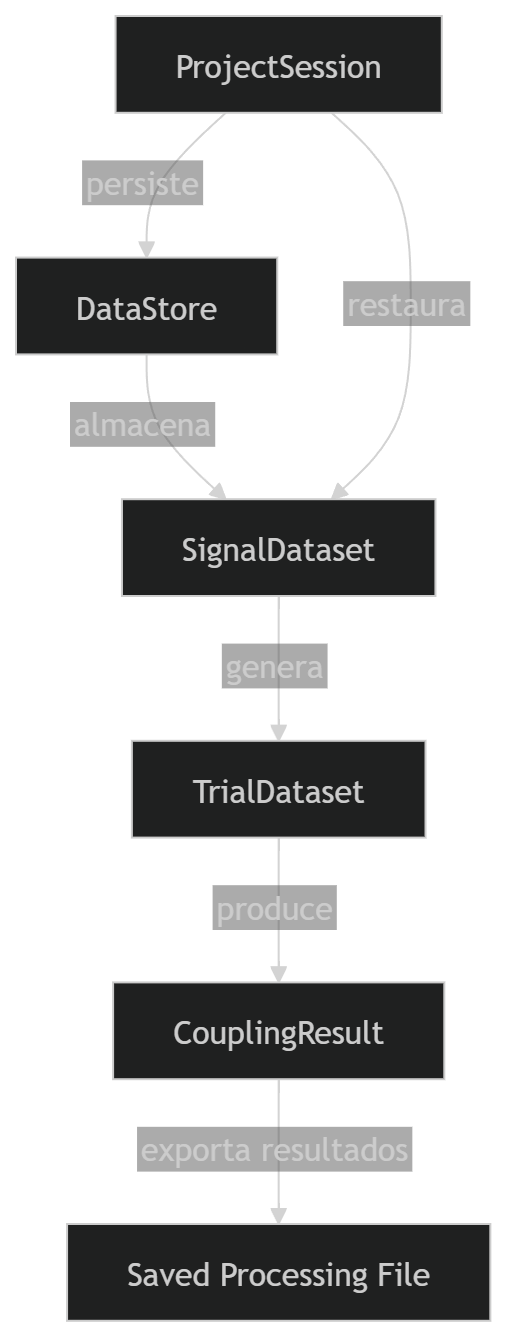
\includegraphics[width=0.5\linewidth]{diagrama de dominio tesis.png}
    \caption{Modelo conceptual del dominio de Gamma Lab 2.0.
Las entidades representan los componentes centrales de almacenamiento,
procesamiento y persistencia de datos neurofisiológicos.}
    \label{fig:placeholder}
\end{figure}

\subsubsection{DataStore}

\begin{table}[H]
\centering

\begin{tabularx}{\textwidth}{|
>{\columncolor{lightgray2}}p{3.4cm}|
Y|
}

\hline
\textbf{ID} & 1 \\ \hline

\textbf{Elemento} & DataStore \\ \hline

\textbf{Descripción}
&
Entidad responsable de gestionar el almacenamiento interno de señales,
datasets experimentales, resultados analíticos y estructuras de sesión
generadas durante la ejecución del sistema. Centraliza la persistencia
temporal y permanente de la información utilizada por los diferentes
módulos de Gamma Lab 2.0.
\\ \hline

\textbf{Responsabilidades}
&
Administrar el acceso a datos, mantener referencias a datasets activos,
coordinar operaciones de lectura y escritura y facilitar la persistencia
de resultados de análisis neurofisiológicos.
\\ \hline

\textbf{Objetivo}
&
Proporcionar una capa centralizada de administración de datos que reduzca
el acoplamiento entre módulos y facilite la reutilización, persistencia y
recuperación de información experimental.
\\ \hline

\end{tabularx}

\caption{Entidad de dominio -- DataStore}
\label{tab:datastore}

\end{table}

\subsubsection{SignalDataset}

\begin{table}[H]
\centering

\begin{tabularx}{\textwidth}{|
>{\columncolor{lightgray2}}p{3.4cm}|
Y|
}

\hline
\textbf{ID} & 2 \\ \hline

\textbf{Elemento} & SignalDataset \\ \hline

\textbf{Descripción}
&
Representa una señal EEG cargada dentro del sistema junto con la estructura
de información requerida para su procesamiento y análisis. Incluye datos
relacionados con frecuencia de muestreo, canales, metadatos experimentales
y formato del archivo original.
\\ \hline

\textbf{Atributos principales}
&
Nombre de la señal, formato del archivo, frecuencia de muestreo, canales
registrados, unidades físicas, duración temporal y metadatos
experimentales asociados.
\\ \hline

\textbf{Objetivo}
&
Estandarizar la representación interna de señales neurofisiológicas para
garantizar interoperabilidad entre los módulos de visualización,
preprocesamiento y análisis.
\\ \hline

\end{tabularx}

\caption{Entidad de dominio -- SignalDataset}
\label{tab:signaldataset}

\end{table}

\subsubsection{TrialDataset}

\begin{table}[H]
\centering

\begin{tabularx}{\textwidth}{|
>{\columncolor{lightgray2}}p{3.4cm}|
Y|
}

\hline
\textbf{ID} & 3 \\ \hline

\textbf{Elemento} & TrialDataset \\ \hline

\textbf{Descripción}
&
Representa el conjunto estructurado de ensayos (\textit{trials}) derivados
de una señal EEG. Cada ensayo corresponde a un segmento temporal asociado a
un estímulo, marcador o evento experimental específico.
\\ \hline

\textbf{Atributos principales}
&
Canal asociado, frecuencia de muestreo, límites temporales, vector temporal
relativo, matriz de ensayos y parámetros experimentales derivados.
\\ \hline

\textbf{Objetivo}
&
Permitir el procesamiento organizado y eficiente de ensayos experimentales
para análisis temporales, espectrales, tiempo-frecuencia y análisis de
acoplamiento entre frecuencias.
\\ \hline

\end{tabularx}

\caption{Entidad de dominio -- TrialDataset}
\label{tab:trialdataset}

\end{table}

\subsubsection{CouplingResult}

\begin{table}[H]
\centering

\begin{tabularx}{\textwidth}{|
>{\columncolor{lightgray2}}p{3.4cm}|
Y|
}

\hline
\textbf{ID} & 4 \\ \hline

\textbf{Elemento} & CouplingResult \\ \hline

\textbf{Descripción}
&
Entidad encargada de almacenar los resultados generados por el módulo de
análisis de acoplamiento cruzado de frecuencias
(\textit{Cross-Frequency Coupling}). Incluye resultados de PAC de un canal,
PAC inter-canal y coherencia de fase PPC.
\\ \hline

\textbf{Atributos principales}
&
Bandas de frecuencia de fase y amplitud, canales utilizados, trials
seleccionados, tipo de análisis, índice de modulación, histograma de fase,
magnitud y ángulo del vector de acoplamiento, matriz del comodulograma,
parámetros de exportación y referencias a archivos generados.
\\ \hline

\textbf{Responsabilidades}
&
Gestionar resultados PAC y PPC, almacenar métricas derivadas y parámetros
utilizados, facilitar la exportación de análisis y permitir la persistencia
de archivos de salida generados durante el procesamiento de señales
neurofisiológicas.
\\ \hline

\textbf{Objetivo}
&
Persistir resultados analíticos y artefactos derivados del procesamiento EEG
para su visualización, exportación, comparación experimental y reutilización
en sesiones futuras.
\\ \hline

\end{tabularx}

\caption{Entidad de dominio -- CouplingResult}
\label{tab:couplingresult}

\end{table}

\subsubsection{ProjectSession}

\begin{table}[H]
\centering

\begin{tabularx}{\textwidth}{|
>{\columncolor{lightgray2}}p{3.4cm}|
Y|
}

\hline
\textbf{ID} & 5 \\ \hline

\textbf{Elemento} & ProjectSession \\ \hline

\textbf{Descripción}
&
Representa el estado persistente de una sesión de trabajo dentro de Gamma
Lab 2.0, incluyendo archivos cargados, parámetros configurados, análisis
ejecutados, resultados almacenados y ventanas activas.
\\ \hline

\textbf{Atributos principales}
&
Identificador del proyecto, fecha de creación, datasets activos,
configuraciones de análisis, historial de procesamiento y ventanas
abiertas.
\\ \hline

\textbf{Objetivo}
&
Permitir la restauración automática de sesiones y la gestión estructurada
de proyectos experimentales dentro del sistema.
\\ \hline

\end{tabularx}

\caption{Entidad de dominio -- ProjectSession}
\label{tab:projectsession}

\end{table}

\subsection{Suposiciones y dependencias}

La presente sección describe las condiciones asumidas durante el desarrollo
de Gamma Lab 2.0 y las dependencias externas necesarias para garantizar el
funcionamiento adecuado del sistema.

\subsubsection{Suposiciones técnicas}

\begin{itemize}

\item El sistema será ejecutado principalmente sobre sistemas operativos
Windows 10 o superiores en arquitectura de 64 bits.

\item El usuario dispondrá de permisos de lectura y escritura sobre el
sistema de archivos local.

\item Los archivos EEG utilizados estarán en formatos compatibles soportados
por la plataforma (\texttt{.abf}, \texttt{.edf}, \texttt{.bdf} y
\texttt{.mat}).

\item Las señales utilizadas para el análisis PAC tendrán al menos un trial
válido.

\item Las señales utilizadas para PAC inter-canal y PPC tendrán al menos dos
canales con trials generados.

\item Las bandas de frecuencia seleccionadas para el análisis se encontrarán
por debajo de la frecuencia de Nyquist.

\item El entorno Python contará con las dependencias científicas requeridas
por los módulos de procesamiento.

\item El equipo de ejecución dispondrá de recursos computacionales suficientes
para manipular señales EEG de gran tamaño.

\item Los módulos desarrollados por terceros respetarán la arquitectura
modular y las interfaces definidas por Gamma Lab.

\end{itemize}

\subsubsection{Suposiciones sobre el usuario}

\begin{itemize}

\item El usuario posee conocimientos básicos o intermedios sobre análisis de
señales EEG y neurofisiología computacional.

\item El usuario comprende conceptos relacionados con análisis temporal,
frecuencial y tiempo-frecuencia.

\item El usuario tiene experiencia básica utilizando interfaces gráficas de
escritorio orientadas a análisis científico.

\item El usuario es capaz de interpretar gráficas, espectros, comodulogramas,
histogramas de fase y resultados estadísticos derivados del sistema.

\item El usuario posee conocimientos básicos de inglés técnico para
comprender terminología científica y nombres de librerías.

\end{itemize}

\subsubsection{Dependencias externas y del sistema}

\begin{itemize}

\item El sistema depende de bibliotecas científicas externas como NumPy,
SciPy, MNE, PyWavelets, PyEDFlib, PyABF, Pandas y TensorPAC.

\item La interfaz gráfica depende del framework PySide6 y de los componentes
Qt.

\item El almacenamiento y control de versiones del proyecto depende de Git y
GitHub.

\item La exportación de resultados depende de librerías de visualización y
generación de archivos CSV, Excel, JSON e imágenes.

\item El módulo de análisis PAC depende de las capacidades de procesamiento de
señales proporcionadas por TensorPAC, MNE, NumPy y SciPy.

\item El módulo de paralelización depende de las capacidades de
multiprocesamiento del sistema operativo y del entorno Python.

\end{itemize}




\newpage
\section{REQUERIMIENTOS ESPECÍFICOS}

Este capítulo define los requerimientos específicos de GammaLab 2.0, derivados de las necesidades y brechas identificadas en la primera versión de la herramienta. Los requerimientos se dividen entre funcionales y no funcionales, y establecen las condiciones que deberá cumplir la nueva iteración para materializar la solución propuesta y orientar su posterior implementación y validación.

\subsection{Nomenclatura de Requisitos}

Con el fin de facilitar la trazabilidad y la referencia cruzada entre los distintos documentos que soportan este trabajo, se definió una nomenclatura que distingue los requisitos funcionales de los no funcionales.

Los requisitos funcionales se identifican mediante el prefijo FR-XX-YY, donde XX corresponde al área funcional de Gamma Lab 2.0 a la que se encuentra asociado el requisito y YY corresponde al número consecutivo dentro de dicha área. Esta clasificación busca mantener una correspondencia entre los requisitos y las principales capacidades funcionales involucradas en la evolución de la herramienta, facilitando su seguimiento a lo largo de las diferentes etapas de diseño, desarrollo y validación.

A partir de esta clasificación, los requisitos funcionales se organizan en cuatro áreas:

\begin{itemize}
    \item \textbf{IO} -- Entrada/Salida: agrupa los requisitos relacionados con la carga y persistencia de señales, así como el guardado y la apertura de proyectos, consolidando el manejo de datos como base funcional de la herramienta.
    \item \textbf{UI} -- Interacción general: agrupa los requisitos orientados a mejorar la experiencia de usuario, la edición de la señal y la gestión de trials.
    \item \textbf{WV} -- Wavelet/Escalograma: agrupa los requisitos que expanden y ajustan las capacidades de esta representación tiempo-frecuencia.
    \item \textbf{PAC} -- Acoplamiento fase-amplitud: agrupa los requisitos del nuevo módulo de análisis incorporado en esta iteración, e incluye tanto el acoplamiento intra-canal como el inter-canal y la coherencia de fase.
\end{itemize}

Los requisitos no funcionales se identifican mediante el prefijo \textbf{NFR-X-YY}, donde \textit{X} corresponde a la categoría del modelo FURPS+ y \textit{YY} es el número consecutivo dentro de dicha categoría. Estos requisitos concentran, en particular, los lineamientos orientados a la estabilización y el fortalecimiento arquitectónico de la herramienta. Se identificaron requisitos en cuatro de las categorías del modelo:

\begin{itemize}
    \item \textbf{U} -- Usabilidad
    \item \textbf{P} -- Rendimiento (Performance)
    \item \textbf{R} -- Confiabilidad (Reliability)
    \item \textbf{S} -- Soporte (Supportability)
\end{itemize}

\subsection{Requerimientos Funcionales}

\subsubsection{Módulo IO -- Entrada/Salida}

\begin{longtable}{|p{2.5cm}|p{2.5cm}|p{11cm}|}
\hline
\rowcolor{gray!25}
\textbf{Código} & \textbf{N° Matriz} & \textbf{Especificación} \\
\hline
\endhead

\hline
\endlastfoot

FR-IO-01 & R08 & El sistema debe persistir la señal cargada \\
\hline
FR-IO-02 & R80 & El sistema debe cargar señales en los formatos ABF, EDF y MAT. \\
\hline
FR-IO-03 & R07 & El sistema debe poder guardar un proyecto que registre la ruta y el nombre del archivo de señal de origen junto con el trabajo realizado sobre ella, sin incluir los datos de la señal. Bajo la extension .glab \\
\hline
FR-IO-04 & R78 & El sistema debe abrir un proyecto guardado, restaurando la señal referenciada y el trabajo registrado en él, e informar cuando el archivo de señal referenciado ya no esté disponible. \\
\hline
FR-IO-05 & R05 & El sistema debe exportar los resultados de la sección de análisis en los formatos Excel, CSV, JSON, JPEG, JPG, PNG y TIFF. \\
\hline
FR-IO-06 & R09 & El sistema debe exportar a CSV una única columna de eje X cuando todas las series comparten el mismo eje. \\
\hline
FR-IO-07 & R28 & El sistema debe asignar un nombre de exportación en el que se incluya el nombre de la señal \\

\end{longtable}
\vspace{-0.5em}
\captionof{table}{Requisitos funcionales del módulo IO}
\label{tab:fr-io}

\subsubsection{Módulo UI -- Interacción general}

\begin{longtable}{|p{2.5cm}|p{2.5cm}|p{11cm}|}
\hline
\rowcolor{gray!25}
\textbf{Código} & \textbf{N° Matriz} & \textbf{Especificación} \\
\hline
\endhead

\hline
\endlastfoot

FR-UI-01 & R01 & El sistema debe permitir realizar cortes de la señal \\
\hline
FR-UI-02 & R24 & El sistema debe modificar un trial ya creado \\
\hline
FR-UI-03 & R25 & El sistema debe restablecer a sus valores por defecto todos los parámetros de una funcionalidad mediante un botón Clear, presente en cada funcionalidad que se ejecute con un botón. \\
\hline
FR-UI-04 & R26 & El sistema debe mostrar los valores de los ejes X y Y correspondientes al punto de la señal sobre el que se posiciona el cursor. \\
\hline
FR-UI-05 & R27 & El sistema debe permitir escoger qué trials participan en cada análisis y descartar los que no deban usarse, conservándolos en el conjunto. \\
\hline
FR-UI-06 & R29 & El sistema debe ajustar el tiempo de muestreo \\
\hline
FR-UI-07 & R30 & El sistema debe tener zoom en todas las direcciones \\
\hline
FR-UI-08 & R31 & El sistema debe mostrar el umbral en mV \\
\hline
FR-UI-09 & R32 & El sistema debe mostrar Butterfly explicitamente \\
\hline
FR-UI-10 & R36 & El sistema debe realizar el promedio en todos los trials \\
\hline
FR-UI-11 & R37 & El sistema debe indicar en todo momento en qué trial se está trabajando. \\
\hline
FR-UI-12 & R38 & El sistema debe indicar qué trials participan en cada operación. \\
\hline
FR-UI-13 & R40 & El sistema debe remover un artefacto con medidas \\
\hline
FR-UI-14 & R41 & El sistema debe promediar los trials específicos que el usuario seleccione. \\
\hline
FR-UI-15 & R68 & El sistema debe identificar cada conjunto de trials por la pareja (archivo, canal) y devolver los trials del canal solicitado, sin reemplazarlo por el último generado. \\

\end{longtable}
\vspace{-0.5em}
\captionof{table}{Requisitos funcionales del módulo UI}
\label{tab:fr-ui}

\subsubsection{Módulo WV -- Wavelet/Escalograma}

\begin{longtable}{|p{2.5cm}|p{2.5cm}|p{11cm}|}
\hline
\rowcolor{gray!25}
\textbf{Código} & \textbf{N° Matriz} & \textbf{Especificación} \\
\hline
\endhead

\hline
\endlastfoot

FR-WV-01 & R33 & El sistema debe permitir elegir el tipo de escala del escalograma de wavelet y ajustar el rango de valores representado. \\
\hline
FR-WV-02 & R34 & El sistema debe normalizar el escalograma de wavelet según el método que elija el usuario. \\
\hline
FR-WV-03 & R35 & El sistema debe exportar wavelet en EMF \\

\end{longtable}
\vspace{-0.5em}
\captionof{table}{Requisitos funcionales del módulo WV}
\label{tab:fr-wv}

\subsubsection{Módulo PAC -- Acoplamiento fase-amplitud}

\begin{longtable}{|p{2.5cm}|p{2.5cm}|p{11cm}|}
\hline
\rowcolor{gray!25}
\textbf{Código} & \textbf{N° Matriz} & \textbf{Especificación} \\
\hline
\endhead

\hline
\endlastfoot

FR-PAC-01 & R13 & El sistema debe ejecutar el análisis de acoplamiento fase-amplitud (PAC) sobre una señal electrofisiológica cargada en el sistema. \\
\hline
FR-PAC-02 & R14 & El sistema debe seleccionar la banda de frecuencia correspondiente a la fase para el análisis PAC. \\
\hline
FR-PAC-03 & R15 & El sistema debe seleccionar la banda de frecuencia correspondiente a la amplitud para el análisis PAC. \\
\hline
FR-PAC-04 & R16 & El sistema debe permitir definir el intervalo temporal (o los trials) sobre el cual se ejecutará el análisis PAC. \\
\hline
FR-PAC-05 & R17 & El sistema debe calcular, para la banda de fase seleccionada y el rango de amplitud seleccionado, un mapa de acoplamiento fase-frecuencia mediante transformada \\
\hline
FR-PAC-06 & R18 & El sistema debe representar los resultados del análisis PAC mediante un mapa fase-frecuencia (fase en el eje X, frecuencia de amplitud en el eje Y). \\
\hline
FR-PAC-07 & R19 & El sistema debe representar la distribución de amplitud en función de la fase (histograma de fase) obtenida durante el análisis PAC. \\
\hline
FR-PAC-08 & R20 & El sistema debe calcular y mostrar el valor del vector de acoplamiento medio (magnitud y ángulo) derivado del histograma de fase. \\
\hline
FR-PAC-09 & R21 & El sistema debe exportar los resultados numéricos del análisis PAC de un canal. \\
\hline
FR-PAC-10 & R22 & El sistema debe exportar las representaciones gráficas generadas durante el análisis PAC de un canal. \\
\hline
FR-PAC-11 & R23 & El sistema debe almacenar los parámetros utilizados en cada ejecución del análisis PAC junto con sus resultados. \\
\hline
FR-PAC-12 & R60 & El sistema debe permitir seleccionar dos canales de la misma señal: uno como fuente de fase y otro como fuente de amplitud. \\
\hline
FR-PAC-13 & R61 & El sistema debe calcular el mapa de acoplamiento fase-frecuencia entre el canal de fase y el canal de amplitud seleccionados. \\
\hline
FR-PAC-14 & R62 & El sistema debe representar los resultados del análisis PAC inter-canal con las mismas visualizaciones que el PAC de un canal. \\
\hline
FR-PAC-15 & R63 & El sistema debe permitir seleccionar dos canales y un rango de frecuencias para calcular la coherencia de fase entre ellos. \\
\hline
FR-PAC-16 & R64 & El sistema debe representar la coherencia de fase mediante un mapa tiempo-frecuencia. \\
\hline
FR-PAC-17 & R65 & El sistema debe exportar los resultados numéricos del análisis PAC inter-canal y de coherencia de fase (PPC). \\
\hline
FR-PAC-18 & R66 & El sistema debe exportar las representaciones gráficas del análisis PAC inter-canal y de coherencia de fase (PPC) como imagen. \\
\hline
FR-PAC-19 & R75 & El sistema debe segmentar la señal filtrada en la banda de frecuencia rápida tomando cada ciclo de la onda lenta como una época, y superponer todas las épocas en una misma gráfica de tipo butterfly con la fase del ciclo lento en el eje X. \\
\hline
FR-PAC-20 & R76 & El sistema debe aplicar sobre la señal activa un filtro Butterworth pasa-banda de fase cero, con frecuencia de corte inferior, frecuencia de corte superior y orden configurables por el usuario. \\

\end{longtable}
\vspace{-0.5em}
\captionof{table}{Requisitos funcionales del módulo PAC}
\label{tab:fr-pac}

\subsection{Requerimientos No Funcionales}

\subsubsection{Categoría U -- Usabilidad}

\begin{longtable}{|p{2.5cm}|p{2.5cm}|p{11cm}|}
\hline
\rowcolor{gray!25}
\textbf{Código} & \textbf{N° Matriz} & \textbf{Especificación} \\
\hline
\endhead

\hline
\endlastfoot

NFR-U-01 & R02 & El sistema debe diferenciar los mensajes informativos, de advertencia y de error, usando el nivel de severidad que corresponda a cada situación. \\
\hline
NFR-U-02 & R03 & El sistema debe mostrar el resultado de la operación en la misma pantalla en la que se realizo \\
\hline
NFR-U-03 & R04 & Toda operación que tome más de 1 segundo debe mostrar retroalimentación visual de progreso \\
\hline
NFR-U-04 & R06 & El sistema debe contar con iconos para cada funcionalidad importante \\
\hline
NFR-U-05 & R10 & EL sistema debe darle una bienvenida a usuarios nuevos \\
\hline
NFR-U-06 & R12 & El sistema debe comunicar el cierre de un proyecto \\
\hline
NFR-U-07 & R42 & El sistema debe mostrar una descripción emergente del propósito de cada control, en cada funcionalidad que se ejecute con un botón. \\
\hline
NFR-U-08 & R43 & El sistema debe mostrar todas las funcionalidades de edición en Home. \\
\hline
NFR-U-09 & R44 & El sistema debe mostrar una pantalla de inicio mientras carga los recursos de arranque. \\

\end{longtable}
\vspace{-0.5em}
\captionof{table}{Requisitos no funcionales de la categoría Usabilidad}
\label{tab:nfr-u}

\subsubsection{Categoría P -- Rendimiento}

\begin{longtable}{|p{2.5cm}|p{2.5cm}|p{11cm}|}
\hline
\rowcolor{gray!25}
\textbf{Código} & \textbf{N° Matriz} & \textbf{Especificación} \\
\hline
\endhead

\hline
\endlastfoot

NFR-P-01 & R11 & El sistema debe liberar la memoria de la señal activa y sus derivados al cerrarse el proyecto activo, ya sea por cierre explícito o por la carga de una nueva señal. \\
\hline
NFR-P-02 & R45 & El sistema debe liberar, al salir de cada módulo, los elementos gráficos y los datos pesados que mantenía en memoria, sin limitarse a ocultarlos de la pantalla. \\
\hline
NFR-P-03 & R47 & El sistema debe cargar el archivo de señal en un tiempo máximo de 2 segundos, contados desde que inicia la lectura hasta que la señal aparece en pantalla, sobre el hardware de referencia del laboratorio. \\
\hline
NFR-P-04 & R48 & El sistema debe completar el cómputo de Wavelet sobre una señal en $\leq$ 10 segundos \\
\hline
NFR-P-05 & R49 & El sistema debe renderizar al menos 3 canales simultáneamente sin que la tasa de refresco caiga por debajo de 24 FPS durante interacción de zoom o desplazamiento, sobre el hardware de referencia del laboratorio. \\
\hline
NFR-P-06 & R50 & El sistema debe completar el cambio entre módulos de análisis en $\leq$ 500 ms manteniendo la señal activa en memoria, sin recargarla desde disco. \\
\hline
NFR-P-07 & R51 & El sistema debe exportar tablas de resultados (CSV, Excel) de hasta 100,000 filas en menos de 2 segundos. \\
\hline
NFR-P-08 & R52 & El sistema debe liberar la memoria asociada a una señal previamente cargada en menos de 1 segundo tras confirmarse la carga de una nueva señal, evitando el crecimiento acumulativo \\
\hline
NFR-P-09 & R53 & El sistema debe completar su cierre, liberando los recursos gráficos, la memoria y los procesos que tenía abiertos, en menos de 3 segundos. \\
\hline
NFR-P-10 & R55 & El sistema debe mantener la interfaz responsiva, con respuesta $\leq$ 0.3 s ante las interacciones, incluso mientras se ejecuta en segundo plano un análisis de frecuencia o de tiempo-frecuencia. \\
\hline
NFR-P-11 & R56 & El sistema debe completar el promedio de todos los trials en $\leq$ 1 segundo para un archivo típico de hasta 50 trials. \\
\hline
NFR-P-12 & R57 & El sistema debe completar la exportación de una gráfica individual en un tiempo máximo de 1 segundo cuando el formato es una imagen rasterizada, y de 3 segundos cuando es vectorial. \\
\hline
NFR-P-13 & R59 & El sistema debe construir las representaciones gráficas de las señales y de los resultados mediante conversiones en bloque, sin recorrer los datos elemento por elemento. \\
\hline
NFR-P-14 & R71 & El sistema debe ejecutar a través del servicio de tareas del núcleo, fuera del hilo de la interfaz, toda operación de cómputo de los plugins: la carga de señal, el corte de trials, el filtrado, la eliminación de artefactos, los análisis de frecuencia individuales y promediados, el promedio de trials, el ERP y los análisis de tiempo-frecuencia individuales y promediados. \\
\hline
NFR-P-15 & R73 & El sistema debe limitar a 2000 puntos por serie y 200 curvas simultáneas en pantalla, submuestreando solo la representación visual sin alterar los datos. \\
\hline
NFR-P-16 & R74 & El sistema debe ejecutar el análisis PAC a través del servicio de tareas del núcleo y completar un comodulograma de hasta 20×20 pares de bandas en un tiempo máximo de 30 s, permitiendo su cancelación. \\
\hline
NFR-P-17 & R81 & El sistema debe quedar listo para usarse en un tiempo máximo de 8 segundos desde que se ejecuta, sobre el hardware de referencia del laboratorio. \\

\end{longtable}
\vspace{-0.5em}
\captionof{table}{Requisitos no funcionales de la categoría Rendimiento}
\label{tab:nfr-p}

\subsubsection{Categoría R -- Confiabilidad}

\begin{longtable}{|p{2.5cm}|p{2.5cm}|p{11cm}|}
\hline
\rowcolor{gray!25}
\textbf{Código} & \textbf{N° Matriz} & \textbf{Especificación} \\
\hline
\endhead

\hline
\endlastfoot

NFR-R-01 & R46 & El sistema debe garantizar la terminación y liberación de todo hilo trabajador del servicio de tareas cuando se detiene el plugin que originó la tarea o cuando esta se cancela, incluso si el cómputo sigue en curso. \\
\hline
NFR-R-02 & R54 & El sistema debe sincronizar el acceso al estado compartido de la sesión cuando varias operaciones se ejecuten a la vez, de modo que un solo propietario escriba cada dato. \\
\hline
NFR-R-03 & R58 & El sistema debe retirar los detectores de eventos registrados sobre las gráficas al salir de cada módulo. \\
\hline
NFR-R-04 & R72 & El sistema debe reutilizar la representación gráfica ya construida de una señal mientras sus datos no cambien, y descartarla de forma explícita cuando se modifiquen. \\
\hline
NFR-R-05 & R79 & El sistema no debe modificar la señal cargada ni los trials originales. Toda operación de preprocesamiento debe registrar su resultado como un conjunto derivado, conservando disponible el conjunto de origen. \\

\end{longtable}
\vspace{-0.5em}
\captionof{table}{Requisitos no funcionales de la categoría Confiabilidad}
\label{tab:nfr-r}

\subsubsection{Categoría S -- Soporte}

\begin{longtable}{|p{2.5cm}|p{2.5cm}|p{11cm}|}
\hline
\rowcolor{gray!25}
\textbf{Código} & \textbf{N° Matriz} & \textbf{Especificación} \\
\hline
\endhead

\hline
\endlastfoot

NFR-S-01 & R39 & El sistema debe generar un ejecutable instalable que registre la extensión .glab en el sistema operativo, de modo que abrir un archivo de proyecto con doble clic inicie la aplicación. \\
\hline
NFR-S-02 & R67 & El sistema debe ofrecer una vía pública y única para leer, modificar e invalidar los trials y sus descartes, sin que ningún módulo alcance la estructura interna de los datos. \\
\hline
NFR-S-03 & R69 & El sistema debe registrar en el núcleo los servicios compartidos de exportación, medición y ajustes, y entregarlos a los módulos con una única instancia de cada uno, sin que ningún módulo los construya por su cuenta. \\
\hline
NFR-S-04 & R70 & El sistema debe ejecutar toda operación de cómputo pesada a través de un servicio de tareas registrado en el núcleo, que gestione la cola, la cancelación y la notificación de progreso. \\
\hline
NFR-S-05 & R77 & El sistema debe permitir incorporar un nuevo plugin de análisis registrándolo en el núcleo y despachando su cómputo por el orquestador, sin modificar el núcleo ni los plugins existentes. \\

\end{longtable}
\vspace{-0.5em}
\captionof{table}{Requisitos no funcionales de la categoría Soporte}
\label{tab:nfr-s}

\newpage
\section{PROCESO INGENIERÍA DE REQUERIMIENTOS}

Esta sección describe el proceso, técnicas y métodos utilizados para la construcción y
administración de los requerimientos del sistema GammaLab~2.0. El objetivo es garantizar
que los requerimientos funcionales y no funcionales se obtengan, documenten, validen y
mantengan de forma consistente durante todo el ciclo de vida del proyecto.

\subsection*{4.1\quad Enfoque General}
\addcontentsline{toc}{subsection}{4.1 Enfoque General}

La ingeniería de requerimientos en GammaLab~2.0 se concibe como un proceso iterativo y
controlado, alineado con el modelo incremental del proyecto. Cada iteración permite refinar,
corregir o ampliar los requerimientos según la retroalimentación obtenida durante el análisis,
diseño, implementación y pruebas.

El proceso involucra tanto al equipo de desarrollo como al cliente final, el Laboratorio de
Señales, asegurando que las necesidades funcionales
y los atributos de calidad se representen de manera verificable. Dado que GammaLab~2.0 es
una versión evolutiva, el proceso parte del análisis de las limitaciones identificadas en la
versión anterior y de los nuevos requerimientos planteados por el cliente.

\subsection*{4.2\quad Actividades del Proceso}
\addcontentsline{toc}{subsection}{4.2 Actividades del Proceso}

El proceso seguido incluye las siguientes actividades principales:

\begin{itemize}[leftmargin=1.5em,itemsep=4pt]
  \item \textbf{Elicitación:} Identificación de necesidades mediante entrevistas con el
        cliente, análisis de las limitaciones de GammaLab~1.0 (SRS v1.1) y revisión técnica
        del dominio de señales EEG y análisis de acoplamiento cruzado de frecuencias.
  \item \textbf{Análisis y refinamiento:} Agrupación, priorización y normalización de
        requerimientos de acuerdo con los cuatro frentes de desarrollo de GammaLab~2.0:
        mejora de UX, paralelización del Kernel, nuevo módulo AC e integración de la
        paralelización con el módulo AC.
  \item \textbf{Documentación:} Registro en el presente SRS utilizando la estructura
        estándar IEEE~29148, garantizando claridad, unicidad y verificabilidad de cada
        requerimiento.
  \item \textbf{Validación:} Revisión con la directora del proyecto en su rol de Product
        Owner y con el cliente, mediante prototipos tempranos y sesiones de revisión
        semanales.
  \item \textbf{Trazabilidad:} Enlace de cada requerimiento con los módulos del sistema,
        el modelo de dominio y los criterios de medición definidos en las fichas de
        especificación.
\end{itemize}

\subsection*{4.3\quad Control de Cambios}
\addcontentsline{toc}{subsection}{4.3 Control de Cambios}

Los requerimientos pueden modificarse a lo largo del desarrollo debido a hallazgos técnicos
o retroalimentación del cliente. Para ello se implementa el siguiente proceso de control:

\begin{itemize}[leftmargin=1.5em,itemsep=4pt]
  \item Canal formal de solicitud de cambio registrado en el repositorio GitHub del
        proyecto.
  \item Evaluación técnica y de esfuerzo por parte del equipo de desarrollo.
  \item Aprobación por parte de la directora del proyecto (Product Owner).
  \item Actualización del SRS, de la distribución de requerimientos y de los
        artefactos afectados.
\end{itemize}

\subsection*{4.4\quad Artefactos Generados}
\addcontentsline{toc}{subsection}{4.4 Artefactos Generados}

\begin{table}[H]
\centering
\renewcommand{\arraystretch}{1.4}

\begin{tabularx}{\textwidth}{
|>{\raggedright\arraybackslash}p{4cm}|
>{\raggedright\arraybackslash}X|
}

\hline

\rowcolor{headergray}

\textbf{Artefacto} &
\textbf{Descripción}
\\ \hline

\rowcolor{lightgray2}
SRS v1.0 &
Presente documento de especificación de requerimientos.
\\ \hline

Acta de requerimientos &
Documento inicial que consolida los requerimientos levantados
durante las sesiones de elicitación.
\\ \hline

\rowcolor{lightgray2}
Distribución de requerimientos &
Tabla de trazabilidad entre módulos y requerimientos
funcionales.
\\ \hline

PMP &
Plan de Administración del Proyecto con cronograma,
roles y gestión de riesgos.
\\ \hline

\rowcolor{lightgray2}
Historial de versiones &
Control de actualizaciones del SRS registrado
en el encabezado del documento.
\\ \hline

\end{tabularx}

\caption{Artefactos generados durante el proceso de ingeniería de requerimientos}
\label{tab:artefactos}

\end{table}
\newpage
\section{PROCESO VERIFICACIÓN}

Esta sección describe el proceso aplicado para verificar y validar los requerimientos
definidos en esta especificación. La verificación en GammaLab~2.0 se desarrolla en estrecha
colaboración con la directora del proyecto en su rol de Product Owner y con el cliente,
el Laboratorio de Señales de la Universidad Nacional de Colombia.

\subsection*{5.1\quad Participación del Cliente}
\addcontentsline{toc}{subsection}{5.1 Participación del Cliente}

El proceso de verificación cuenta con la supervisión de la directora del proyecto, quien
actúa como enlace técnico con el Laboratorio de Señales. Su rol es fundamental para:

\begin{itemize}[leftmargin=1.5em,itemsep=3pt]
  \item Validar los requerimientos durante su construcción, asegurando que reflejen las
        necesidades reales del laboratorio.
  \item Proporcionar retroalimentación técnica desde la perspectiva del dominio EEG y del
        análisis de acoplamiento cruzado de frecuencias.
  \item Aceptar o rechazar funcionalidades implementadas en cada iteración de desarrollo.
  \item Asegurar que los resultados y herramientas generadas sean coherentes con los
        procedimientos experimentales del laboratorio.
\end{itemize}

\subsection*{5.2\quad Dinámica de Verificación}
\addcontentsline{toc}{subsection}{5.2 Dinámica de Verificación}

El proceso de verificación se desarrolla mediante ciclos iterativos de revisión. En cada
ciclo se presentan los avances implementados, incluyendo:

\begin{itemize}[leftmargin=1.5em,itemsep=3pt]
  \item Funcionalidades desarrolladas en la iteración correspondiente.
  \item Correcciones a requerimientos previamente observados.
  \item Comportamientos de la interfaz y flujos completos de uso.
  \item Validación directa sobre datos reales del laboratorio, cuando aplica.
\end{itemize}

Durante estas sesiones, el cliente aprueba, solicita ajustes o rechaza funcionalidades
según su alineación con los objetivos científicos del proyecto. Esta dinámica permite
mantener los requerimientos actualizados, claros y técnicamente viables a lo largo del
ciclo de desarrollo.

\subsection*{5.3\quad Mecanismo de Control y Seguimiento}
\addcontentsline{toc}{subsection}{5.3 Mecanismo de Control y Seguimiento}

Para garantizar trazabilidad completa, el equipo utiliza un flujo controlado mediante ramas
en el repositorio oficial de GitHub. Cada avance del sistema se gestiona bajo las siguientes
prácticas:

\begin{itemize}[leftmargin=1.5em,itemsep=3pt]
  \item Creación de ramas específicas por funcionalidad o corrección
        (\texttt{feature/nombre-funcionalidad}).
  \item Revisión interna por parte del equipo antes de su presentación al cliente.
  \item Retroalimentación del cliente y ajustes sobre la misma rama.
  \item Aprobación final y posterior integración (\emph{merge}) al repositorio principal.
\end{itemize}

Este mecanismo permite asociar cada requerimiento con su evidencia de implementación y con
el historial de revisiones, asegurando un proceso verificable y consistente.

\subsection*{5.4\quad Criterios de Verificación por Tipo de Requerimiento}
\addcontentsline{toc}{subsection}{5.4 Criterios de Verificación por Tipo de Requerimiento}



\begin{table}[H]
\centering

\renewcommand{\arraystretch}{1.4}

\begin{tabularx}{\textwidth}{|
>{\raggedright\arraybackslash\bfseries}p{4cm}|
X|
}

\hline

\rowcolor{headergray}

\textbf{Tipo} &
\textbf{Criterio de verificación}
\\ \hline

\rowcolor{lightgray2}
Requerimientos funcionales &
Prueba directa de la funcionalidad sobre datos reales del laboratorio,
con aprobación explícita del cliente.
\\ \hline

Requerimientos de desempeño &
Medición de tiempos de ejecución con señales de referencia y comparación
contra los umbrales definidos.
\\ \hline

\rowcolor{lightgray2}
Requerimientos no funcionales &
Revisión de código, pruebas de carga y validación de comportamiento
bajo condiciones adversas.
\\ \hline

Requerimientos de persistencia &
Verificación de restauración correcta de sesiones tras cierre y
reapertura de la aplicación.
\\ \hline

\rowcolor{lightgray2}
Paralelización (módulo PL) &
Comparación de tiempos de análisis secuencial vs.\ paralelo sobre un
conjunto de \textit{trials} de referencia, verificando que la GUI
permanezca responsiva.
\\ \hline

Módulo PAC &
Validación del cálculo PAC contra resultados de referencia conocidos,
con revisión de la gráfica del comodulograma por parte del cliente.
\\ \hline

\end{tabularx}

\caption{Criterios de verificación por tipo de requerimiento}
\label{tab:criterios_verificacion}

\end{table}

\subsection*{5.5\quad Resultado del Proceso}
\addcontentsline{toc}{subsection}{5.5 Resultado del Proceso}

La verificación continua con el cliente, junto con el control basado en ramas y revisiones
iterativas, garantiza que:

\begin{itemize}[leftmargin=1.5em,itemsep=3pt]
  \item Cada requerimiento cuente con una validación explícita antes de considerarse
        implementado.
  \item Los cambios se gestionen de forma transparente y ordenada mediante el historial
        de Git.
  \item El sistema final cumpla con las expectativas científicas y funcionales del
        Laboratorio de Señales
  \item La trazabilidad entre requerimientos, diseño y código se mantenga durante todo
        el desarrollo del proyecto.
\end{itemize}

\newpage
\section{ANEXOS}

\end{document}